\documentclass[10pt,twocolumn,letterpaper]{article}
\usepackage[margin=0.7in,columnsep=0.25in]{geometry}
\usepackage[T1]{fontenc}
\usepackage{lmodern}
\usepackage{microtype}
\usepackage{graphicx}
\usepackage{booktabs}
\usepackage{subcaption}
\usepackage{enumitem}
\usepackage[hidelinks]{hyperref}
\usepackage{xcolor}

\graphicspath{{figures/}}
\setlist{nosep,leftmargin=1.2em}
\setlength{\textfloatsep}{8pt plus 2pt}
\setlength{\floatsep}{6pt plus 2pt}
\setlength{\abovecaptionskip}{3pt}
\captionsetup{font=small,labelfont=bf}
\captionsetup[sub]{font=footnotesize}
\newcommand{\task}[1]{\texttt{\small #1}}

\title{\vspace{-1.2em}Spatial Reasoning by Construction: A Block Benchmark with Provable No-Solution Cases\vspace{-0.4em}}
\author{Ammaar Alam \quad Erik Dyer\\
\small COS 597C, Princeton University, Fall 2026\\
\small Repository: \url{https://github.com/Ammaar-Alam/project-01-spatial-reasoning}}
\date{\vspace{-2em}}

\begin{document}
\maketitle

\begin{abstract}
Most spatial reasoning benchmarks for vision language models are multiple choice, so a model can guess, we never see the shape it had in mind, and a question with no valid answer is awkward to pose. We built a benchmark where the model answers by \emph{constructing} the final 3D structure: a complete list of occupied grid cells, graded by exact match against every accepted answer. Tasks cover rebuilding and rotating shapes from pictures, combining views, stick-frame and three-view puzzles, and repairs; 28 of the 118 evaluated tasks have no solution. Across ten settings of six models from three labs, the best solve 56 of our first 64 tasks and all 30 of a harder follow-up set. Yet when a single picture hides a cell, nine of ten settings always built a definite structure and never said the picture was insufficient. A second picture showing the cell empty, or one warning sentence, fixed this only for the three or four strongest settings.
\end{abstract}

\section{Motivation}
Spatial benchmarks such as BLINK~\cite{blink}, SpatialEval~\cite{spatialeval} and 3DSRBench~\cite{3dsr} mostly score a choice among given options. That format has three costs: chance accuracy is high, a wrong answer reveals little about the model's internal picture of the scene, and it cannot naturally ask a question whose honest answer is ``this cannot be determined.'' Mental rotation~\cite{shepard} and multi-view reconstruction are better tested by asking for the object itself.

We ask: \emph{when a model must build its answer, how well does it read and transform 3D shapes, and does it notice when the input does not determine the shape?} The second half matters for agents that act on visual input. Abstention work on unanswerable questions~\cite{vizwiz,abstention} mostly uses text or natural photos; our renders let us \emph{prove} which cells a camera cannot see, so the no-solution label is exact rather than annotated.

\section{Benchmark design}

\paragraph{One episode.} A model receives one system prompt and one task message, and replies once. The system prompt fixes the coordinate convention (integer $x,y,z$; $y$ up; $y{=}0$ the floor) and the reply format. The task message holds the instruction, a sentence describing where each camera sits and which way the axes run in the picture, the grid bounds, the starting blocks as JSON (or ``empty''), any rules (edit budget, exact block count, protected cells, add-only or remove-only), and the task's images. There are no tools, examples, retries or feedback. Table~\ref{tab:families} and Figure~\ref{fig:inputs} list exactly what each family sends.

\paragraph{Images.} Every image is a still $1024{\times}768$ PNG rendered by our own Three.js editor with fixed lighting and framing; no task includes video or animation. Perspective pictures are taken from above the $(+x,+z)$ corner, plus the opposite $(-x,-z)$ corner for two-picture tasks; three-view tasks use orthographic front, side and top views. The turning renders we use for inspecting answers are produced from saved replies after grading and are never sent to a model. Set C (below) instead uses hand-drawn diagrams, and 8 of its tasks are text only.

\begin{table}[t]
\centering\small
\setlength{\tabcolsep}{3pt}
\begin{tabular}{@{}l r p{5.3cm}@{}}
\toprule
Family & Tasks & The model receives \\
\midrule
\task{rebuild} & 11 & 1 perspective picture, empty grid \\
\task{rotate} & 19 & 1 picture and a stated turn, tip, flip or mirror \\
\task{twoview} & 18 & 2 pictures from opposite corners \\
\task{hinted} & 6 & 1 picture and a warning sentence \\
\task{sticks} & 19 & a frame as up to 208 starting blocks and 1 picture \\
\task{views} & 17 & front, side and top orthographic pictures \\
\task{repair} & 4 & 1--2 pictures and a block list with errors \\
\midrule
Set C & 24 & count maps, piece layers or camera diagrams (0--10 images), or text only, plus JSON \\
\bottomrule
\end{tabular}
\caption{Inputs per family. Sets A and B (94 tasks) use the first seven rows; every task message also states the grid bounds, camera placement and rules.}
\label{tab:families}
\end{table}

\begin{figure*}[t]
\centering
\begin{subfigure}[b]{0.12\textwidth}\centering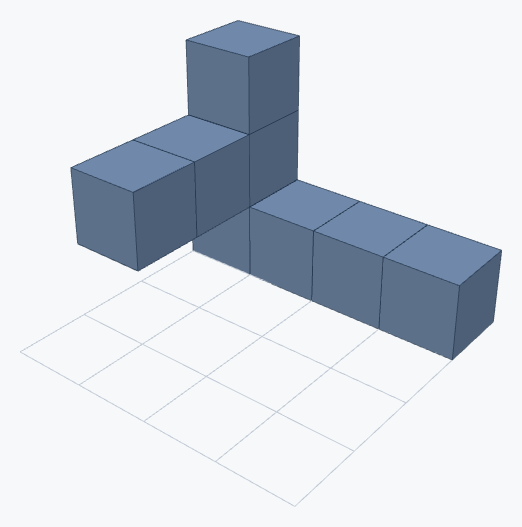
\includegraphics[height=2.0cm]{hook.png}\caption{one picture}\end{subfigure}\hfill
\begin{subfigure}[b]{0.22\textwidth}\centering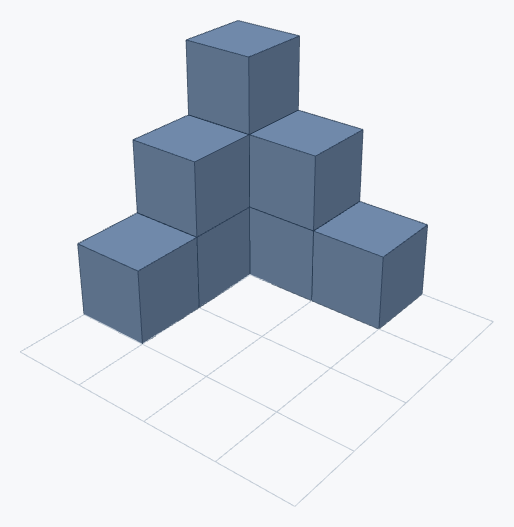
\includegraphics[height=1.7cm]{corner-angled.png}\,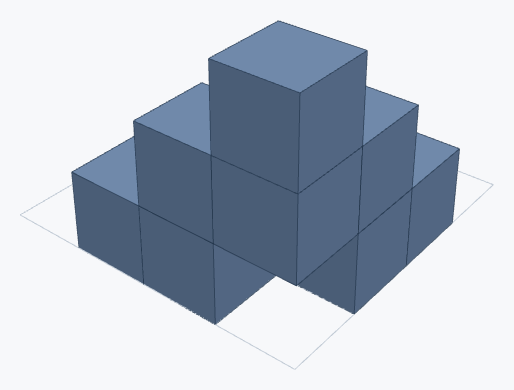
\includegraphics[height=1.7cm]{corner-behind.png}\caption{two pictures}\end{subfigure}\hfill
\begin{subfigure}[b]{0.25\textwidth}\centering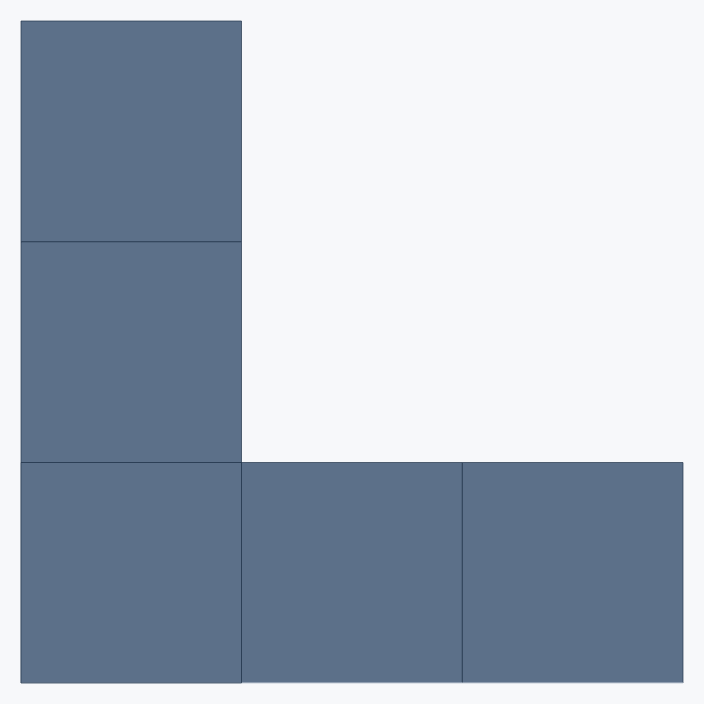
\includegraphics[height=1.3cm]{ell-front.png}\,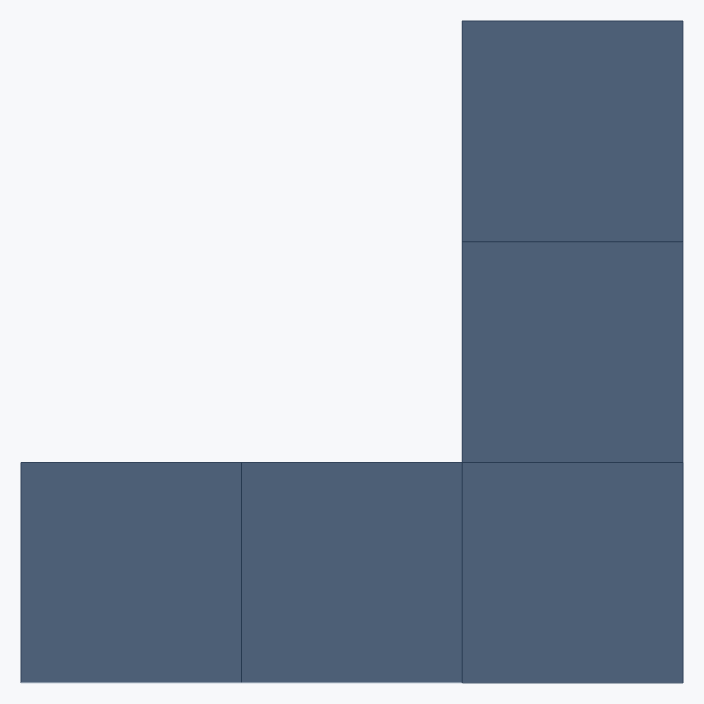
\includegraphics[height=1.3cm]{ell-side.png}\,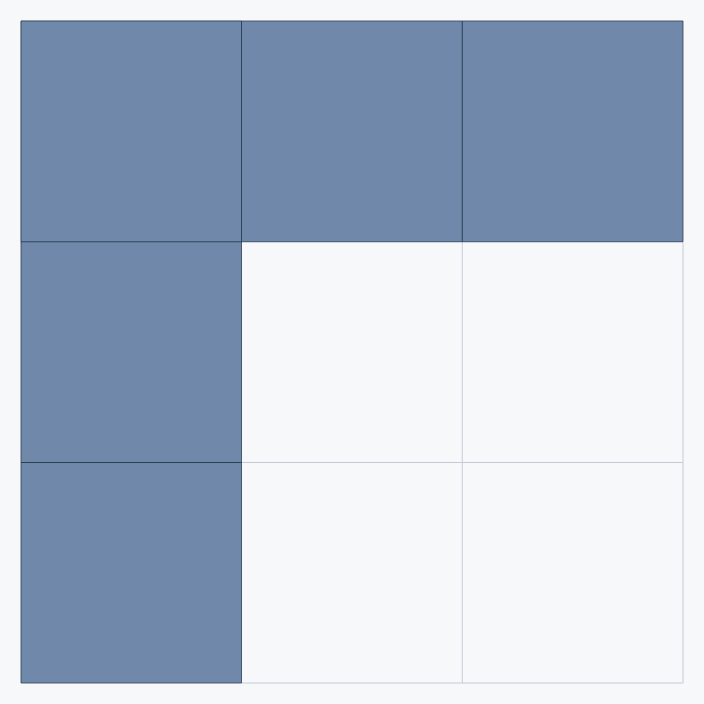
\includegraphics[height=1.3cm]{ell-top.png}\caption{three views}\end{subfigure}\hfill
\begin{subfigure}[b]{0.12\textwidth}\centering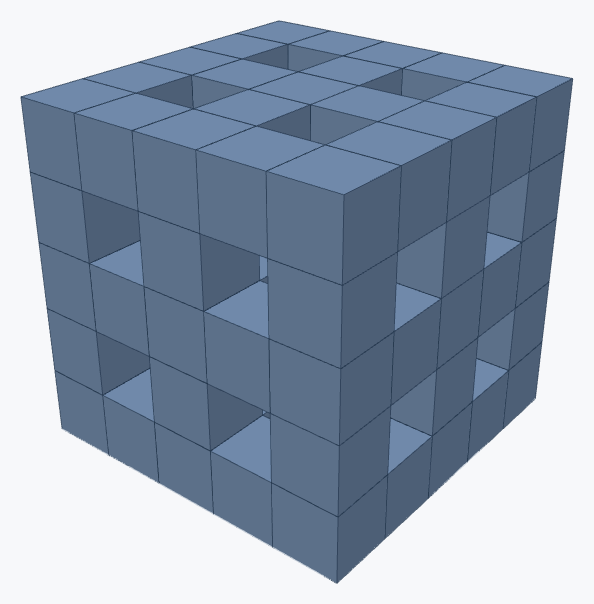
\includegraphics[height=2.0cm]{frame.png}\caption{stick frame}\end{subfigure}\hfill
\begin{subfigure}[b]{0.11\textwidth}\centering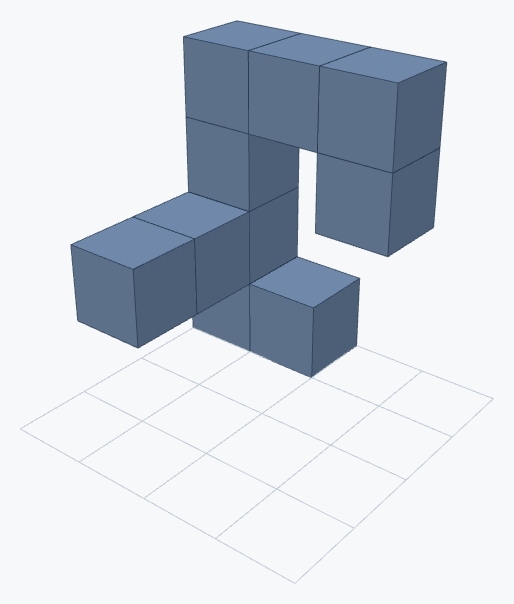
\includegraphics[height=2.0cm]{tree.png}\caption{repair}\end{subfigure}\hfill
\begin{subfigure}[b]{0.12\textwidth}\centering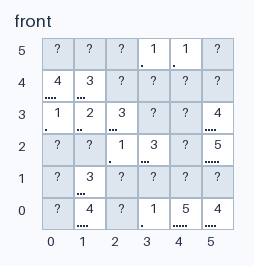
\includegraphics[height=2.0cm]{countmap.png}\caption{count map}\end{subfigure}
\caption{Images as the model receives them (cropped). (d) also arrives as a JSON list of every block; (e) arrives with a faulty block list to fix; (f) is part of one of three diagram pages in a Set C count-map task.}
\label{fig:inputs}
\end{figure*}

\paragraph{Reply and grading.} The reply must be exactly one JSON object, optionally inside one \verb|```json| fence: either \verb|{"status":"solved","blocks":[...]}| with every final block, or \verb|{"status":"impossible","reason":"..."}|. Anything else (extra prose, a second object, extra fields, non-integer or out-of-bounds cells, duplicates) fails; nothing is repaired. A solved reply passes when it obeys every rule and its cell set equals the reference or one of the listed alternatives, in any order. On a no-solution task only an \texttt{impossible} reply passes; the reason is stored but not graded. Both reply options are offered on every task.

\paragraph{Answer keys and no-solution labels.} Keys are computed, not drawn by hand. Rotated targets are produced by applying the turn to the source cells, and every placement that fits the grid is accepted, since prompts say the shape may sit anywhere. Visibility is proved by rendering each cell alone, white among black blocks, from a copy of the task camera and counting its pixels: a solvable picture task needs every cell, filled or empty, to show at least 400 pixels in some view, and each ``hidden'' task names an empty cell that shows 0 in every view given. Stick-frame and three-view keys enumerate every final structure meeting the counts, so a no-solution label means none exists. Each task file holds its prompt, images, rules, reference and alternatives, and \texttt{pnpm tasks:check} grades the reference and alternatives with the real grader.

\paragraph{The hidden-block test.} Six shapes have one cell that a single picture cannot show. Three of them are asked three ways: one picture (no solution), the same picture plus a second from the opposite corner that shows the cell empty (solvable), and one picture with the sentence ``Parts of a structure can be hidden from the camera. If the picture leaves any block in doubt, say the task cannot be done'' (no solution). Three solvable shapes carry the same warning, so a model cannot score by always declining.

\paragraph{Harness.} \texttt{pnpm bench} sends each attempt as one request through the Anthropic, OpenAI, Gemini or OpenRouter API, with OpenRouter fallback disabled. Each finished attempt is appended to \texttt{records.jsonl} with the raw reply, stop reason, usage, latency and grade; \texttt{run.json} stores the prompts, settings, a hash of every task and of the code. Provider failures are saved as errors, not graded, and rerunning the same command retries only those. \texttt{pnpm editor} serves the block editor used to build tasks and a viewer that draws each saved answer over the closest correct structure.

\section{Experimental setup}
\textbf{Set A} (64 tasks, 17 no-solution) is the main suite. \textbf{Set B} (30 tasks, 5 no-solution) was added after Set A neared the ceiling: diagonal and three-step turns, boxes with gaps to fill, contradictory picture pairs, move-$K$-sticks puzzles, three-view tasks where every block must rest on another, repairs, and five shapes of 20--21 blocks in a $5^3$ grid. \textbf{Set C} (24 tasks, 6 no-solution) is a separately authored set of harder construction puzzles: packing eight pieces into a cavity, rebuilding from nine count maps with two wrong, ten rounds of camera-relative edits, and minimum connect and separate puzzles.

We ran ten settings: GPT-6.1 Sol, GPT-6 Sol and GPT-6 Luna at high effort, GPT-6 Astra at low and high, Claude Opus 5.5 at low and high, Gemini 4 Argon at high, and Gemini 3.8 Flash at low and high. Output limits were 128K tokens (65,536 for Flash), sampling at API defaults, one attempt per task. Opus ran through OpenRouter, where effort maps to a thinking budget; on 37 Set A tasks it scored within one task of direct Anthropic runs. Argon replies past 32,768 tokens are continued with the API's continuation token, which needed a runner change. All runs in Table~\ref{tab:main} except Argon's cost roughly \$120 at list prices.

\section{Results}

\begin{table*}[t]
\centering\small
\setlength{\tabcolsep}{4.6pt}
\resizebox{\textwidth}{!}{\begin{tabular}{@{}l ccc cccc c cc@{}}
\toprule
& \multicolumn{3}{c}{Set A} & \multicolumn{4}{c}{Hidden-block test (in Set A)} & Set B & \multicolumn{2}{c}{Set C} \\
\cmidrule(lr){2-4}\cmidrule(lr){5-8}\cmidrule(lr){9-9}\cmidrule(l){10-11}
Setting & All & Solvable & No sol. & One pic. & Two pics. & Warned, hidden & Warned, solvable & All & Solvable & Wrongly declined \\
& /64 & /47 & /17 & /6 & /3 & /3 & /3 & /30 & /18 & of 18 \\
\midrule
GPT-6 Astra, high & \textbf{56} & 46 & 10 & 0 & 3 & 3 & 3 & \textbf{30} & \textbf{12} & 4 \\
GPT-6.1 Sol, high & \textbf{56} & \textbf{47} & 9 & 0 & 3 & 3 & 3 & \textbf{30} & 11 & 7 \\
Gemini 4 Argon, high & \textbf{56} & 43 & \textbf{13} & \textbf{3} & 3 & 3 & 2 & 27 & 10 & 1 \\
Claude Opus 5.5, high & 51 & 44 & 7 & 0 & 2 & 0 & 3 & 26 & -- & -- \\
GPT-6 Astra, low & 50 & 40 & 10 & 0 & 2 & 3 & 0 & 24 & 4 & 14 \\
GPT-6 Sol, high & 41 & 34 & 7 & 0 & 0 & 1 & 1 & 19 & 3 & 11 \\
Claude Opus 5.5, low & 38 & 30 & 8 & 0 & 0 & 1 & 2 & 15/22 & -- & -- \\
Gemini 3.8 Flash, high & 38 & 31 & 7 & 0 & 0 & 0 & 1 & 13 & 4 & 9 \\
Gemini 3.8 Flash, low & 36 & 29 & 7 & 0 & 0 & 0 & 2 & 11 & 3 & 14 \\
GPT-6 Luna, high & 31 & 24 & 7 & 0 & 0 & 0 & 1 & 14 & 3 & 14 \\
\bottomrule
\end{tabular}}
\caption{Tasks right, one attempt each. ``One pic.'' counts the six one-picture hidden-block tasks answered \texttt{impossible}; ``two pics.'' and ``warned'' are the matched versions described in Section 2. The last column counts \texttt{impossible} replies to solvable Set C tasks. Opus was not run on Set C, and Opus low on only 22 of Set B.}
\label{tab:main}
\end{table*}

\paragraph{Overall.} Table~\ref{tab:main} gives every score. Three settings tie at 56/64 on Set A (95\% Wilson interval 77--94\%), so with one attempt per task, gaps of a few tasks are within noise. Effort matters a great deal for Opus (51 vs.\ 38) and less for Astra (56 vs.\ 50) and Flash (38 vs.\ 36). Across all 118 tasks, Astra high solves 104 and GPT-6.1 Sol 103.

\paragraph{Hidden blocks are filled in, not flagged.} On the six one-picture hidden-block tasks, nine of ten settings returned a definite structure every time, 54 of 54 answers. Only Argon answered \texttt{impossible}, on 3 of 6. The no-solution tasks that rest on counting or fit, by contrast, were caught by nearly everyone: across Sets A and B, every setting got all three stick-frame and at least five of six three-view no-solution tasks right.

\paragraph{Evidence and warnings help only the strongest.} With the second picture showing the cell empty (Figure~\ref{fig:corner}), Astra high, GPT-6.1 Sol and Argon built the visible structure on all three shapes; Opus high and Astra low did so on two; the other five failed all three. The warning sentence made Astra (both efforts), GPT-6.1 Sol and Argon decline all three hidden tasks, so these models can detect the gap when asked to look for it. Astra low then also declined all three solvable controls. Opus high, Flash and Luna did not change.

\begin{figure}[t]
\centering
\begin{subfigure}[b]{0.31\columnwidth}\centering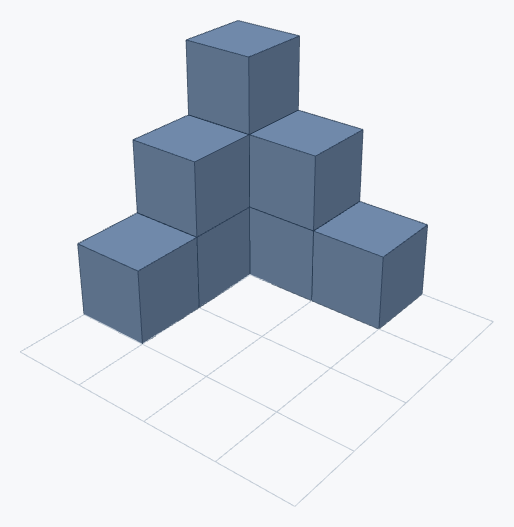
\includegraphics[height=1.9cm]{corner-angled.png}\caption{one picture}\end{subfigure}\hfill
\begin{subfigure}[b]{0.31\columnwidth}\centering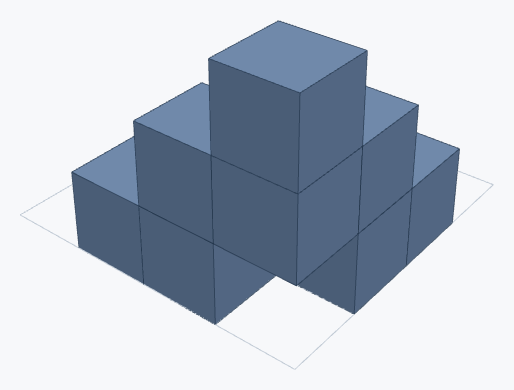
\includegraphics[height=1.9cm]{corner-behind.png}\caption{second picture}\end{subfigure}\hfill
\begin{subfigure}[b]{0.34\columnwidth}\centering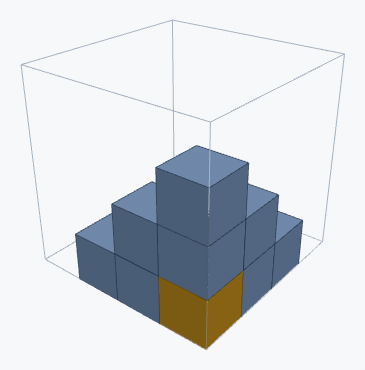
\includegraphics[height=2.0cm]{opus-corner.png}\caption{Opus 5.5 high}\end{subfigure}
\caption{\task{twoview/corner}. The back corner cell is hidden in (a) and visibly empty in (b). Given both, Opus 5.5 high still fills it (amber, seen from behind).}
\label{fig:corner}
\end{figure}

\paragraph{Reading the picture is the main difficulty.} Every setting solved at least 11 of 13 stick-frame tasks, which arrive as JSON blocks, while the 19 solvable rebuild and rotate tasks ranged from 7 (Luna) to 19 (Astra high, GPT-6.1 Sol). The families differ in more than modality, so this suggests rather than shows that image reading drives the gap.

\paragraph{Harder tasks spread the field.} On Set B, Astra high and GPT-6.1 Sol stayed perfect while the rest fell to 11--27. The 20-block shapes read from two pictures separated most: the top two solved all five, Astra low four, Argon and Opus high three each, the rest none. On the two contradictory picture pairs, weaker settings again built a structure rather than declining.

\paragraph{Set C reverses the failure.} On the construction puzzles the best setting solved 12 of 18 solvable tasks, and the dominant error flips: our eight settings answered \texttt{impossible} on 74 of 144 solvable attempts. Argon stopped at its output limit on 10 of 24. A separate run of seven other models through one provider (GLM 5.3 Flash, DeepSeek V4.1 Flash, Qwen 3.7 Flash, Kimi K2.5, MiMo V2.5, Gemini 3.8 Flash, GPT-6 Luna), stored in the repository, scored at most 4 of 18, with 50 of 121 graded solvable replies wrongly declining and 39 of 160 stopping at the output limit. Models overcommit when information is missing and give up when a puzzle is hard but solvable.

\section{What did not work, and limitations}
\begin{itemize}
\item \textbf{Saturation.} Our first 37 tasks were near ceiling for the top settings, which is why Sets B and C exist; Set B is still at ceiling for two settings, so we have no solvable tasks that separate them.
\item \textbf{Strict format.} Opus at low effort often wrote prose before the JSON, failing 7 Set A replies that a lenient parser would read. We kept the strict rule so a score means one clean reply.
\item \textbf{Providers.} Anthropic credit ran out mid-project, so Opus moved to OpenRouter, where effort is a thinking budget rather than Anthropic's setting. OpenRouter sometimes returned an empty reply with no finish reason; these were first graded as invalid until we changed the runner to treat them as errors. GLM 5.3 Flash and DeepSeek V4.1 Flash runs on Set A were left incomplete by repeated upstream failures and are excluded. Argon needed a continuation change to the runner, so its runs carry a different code hash.
\item \textbf{No matched modality test.} Picture and coordinate tasks come from different families, so the image-reading claim is not isolated.
\item \textbf{Scale.} One attempt per task and no intervals per family; six hidden-block shapes and one warning wording; synthetic renders only; no human baseline; no tool use, so models could not compute rotations with code. Set C mixes diagrams and text and was run with unequal output budgets.
\end{itemize}

\section{Conclusion}
Asking models to build their answer makes spatial errors visible and lets a benchmark pose questions that have no answer with a provable label. Frontier settings read and turn small block shapes well, but nine of ten never said a picture was insufficient, and extra evidence or an explicit warning fixed this only for the strongest. Next we will run five attempts per task with intervals, add hidden-block shapes and warning wordings, pair each picture task with a coordinate twin, add solvable tasks the top two miss, and compare against runs with a code tool. Reproduction: \texttt{pnpm install}, \texttt{pnpm check}, then \texttt{pnpm bench -{}-name <run> -{}-models <setting> -{}-tasks <ids>}, with each run's task ids listed in \texttt{results/<run>/run.json}; all replies and grades are in \texttt{results/}.

\small
\begin{thebibliography}{9}\setlength{\itemsep}{0pt}
\bibitem{blink} X.~Fu et al. BLINK: Multimodal large language models can see but not perceive. ECCV, 2024.
\bibitem{spatialeval} J.~Wang et al. Is a picture worth a thousand words? Delving into spatial reasoning for vision language models. NeurIPS, 2024.
\bibitem{3dsr} W.~Ma et al. 3DSRBench: A comprehensive 3D spatial reasoning benchmark. arXiv:2412.07825, 2024.
\bibitem{shepard} R.~N. Shepard and J.~Metzler. Mental rotation of three-dimensional objects. Science 171(3972), 1971.
\bibitem{vizwiz} D.~Gurari et al. VizWiz Grand Challenge: Answering visual questions from blind people. CVPR, 2018.
\bibitem{abstention} P.~Kirichenko et al. AbstentionBench: Reasoning LLMs fail on unanswerable questions. arXiv:2506.09038, 2025.
\end{thebibliography}
\end{document}
